\section{Symulacyjne wyznaczenie odpowiedzi skokowych}
\label{projekt:zad2}

Wyznaczyc symulacyjnie odpowiedzi skokowe procesu dla kilku zmian sygnału sterujacego,
przy uwzglednieniu ograniczen wartosci tego sygnału, jego wartosc na poczatku
eksperymentu wynosi 0. Narysowac te odpowiedzi na jednym rysunku. Narysowac charakterystyke
statyczna procesu y(u). Czy własciwosci statyczne i dynamiczne procesu
sa liniowe?

Odpowiedzi skokowe toru wejście-wyjście zostały wyznaczone
symulacyjnie dla pięciu zmian sygnału sterującego.

\subsection{Odpowiedzi skokowe}
\label{projekt:zad2:odpSkok}

\begin{figure}[H] 
    \centering
    \section{Wyznaczenie odpowiedzi skokowej procesu}
Wyznaczyć odpowiedzi skokowe procesu dla trzech różnych zmian sygnału sterującego
G1 rozpoczynając z punktu pracy. Narysować otrzymane przebiegi na jednym rysunku.
Czy właściwości statyczne obiektu można określić jako (w przybliżeniu) liniowe? Jeśli
tak wyznaczyć wzmocnienie statyczne procesu?

    \caption{Odpowiedzi skokowe obiektu}
    \label{projekt:zad2:odpSkok:figure}
\end{figure}

\newpage

\subsection{Charakterystyka statyczna}
\label{projekt:zad2:charStat}

\begin{figure}[H] 
    \centering
    % This file was created by matlab2tikz.
%
\definecolor{mycolor1}{rgb}{0.00000,0.44700,0.74100}%
%
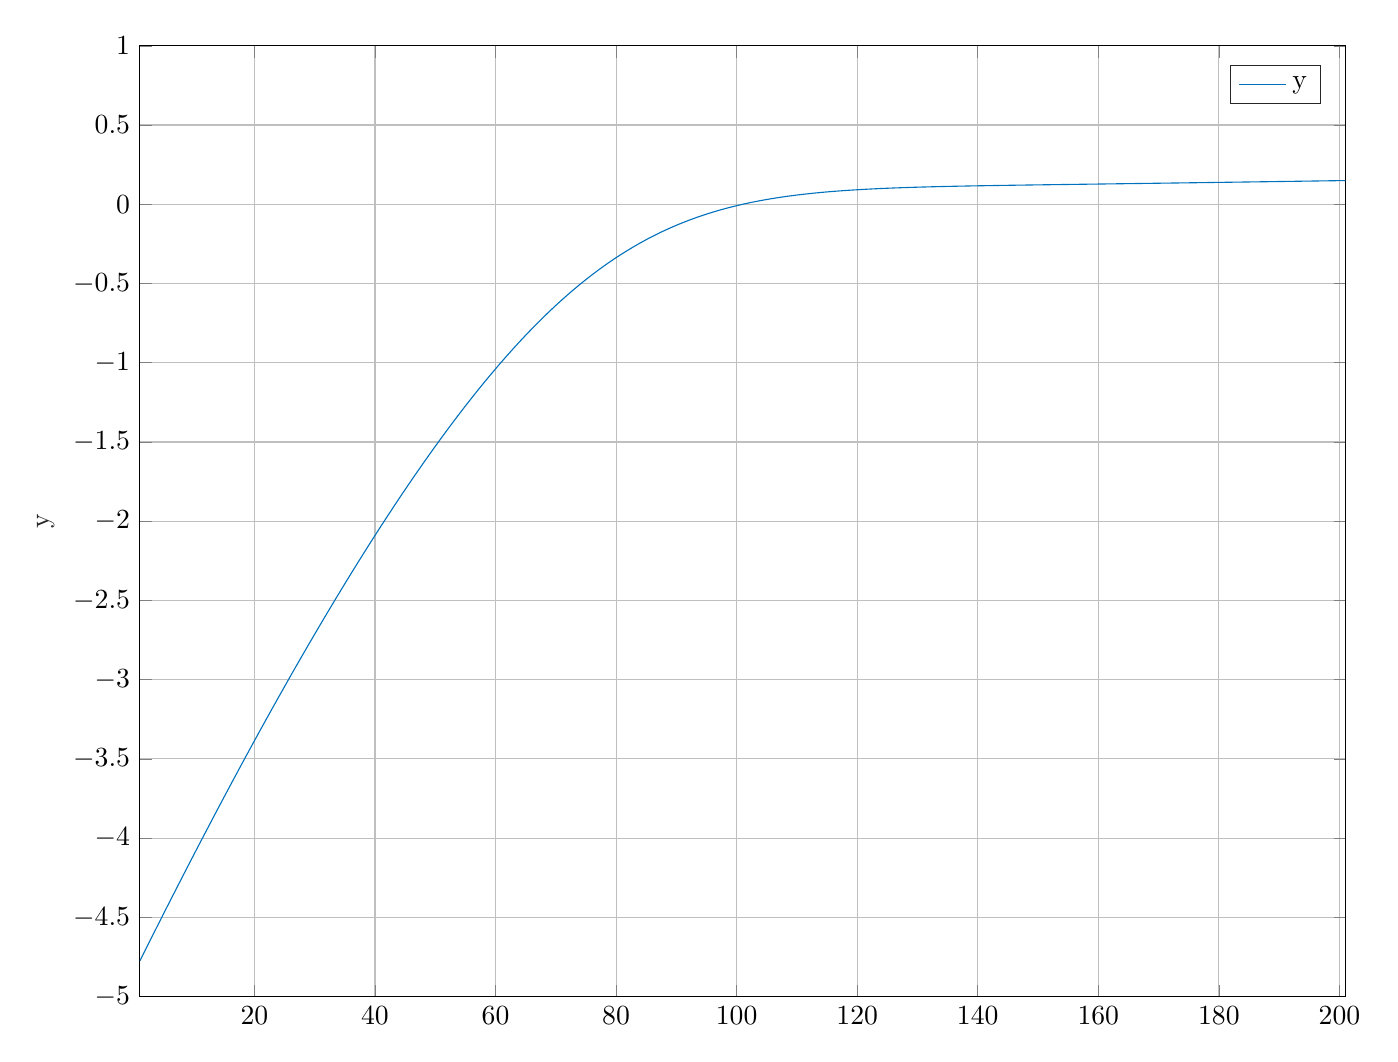
\begin{tikzpicture}

\begin{axis}[%
width=6.028in,
height=4.754in,
at={(1.011in,0.642in)},
scale only axis,
xmin=1,
xmax=201,
ymin=-5,
ymax=1,
ylabel style={font=\color{white!15!black}},
ylabel={y},
axis background/.style={fill=white},
xmajorgrids,
ymajorgrids,
legend style={legend cell align=left, align=left, draw=white!15!black}
]
\addplot [color=mycolor1]
  table[row sep=crcr]{%
1	-4.7747\\
2	-4.6987\\
3	-4.6229\\
4	-4.5474\\
5	-4.4722\\
6	-4.3973\\
7	-4.3228\\
8	-4.2485\\
9	-4.1746\\
10	-4.101\\
11	-4.0278\\
12	-3.955\\
13	-3.8825\\
14	-3.8103\\
15	-3.7386\\
16	-3.6672\\
17	-3.5963\\
18	-3.5257\\
19	-3.4556\\
20	-3.3858\\
21	-3.3165\\
22	-3.2476\\
23	-3.1792\\
24	-3.1112\\
25	-3.0437\\
26	-2.9766\\
27	-2.91\\
28	-2.8438\\
29	-2.7782\\
30	-2.713\\
31	-2.6483\\
32	-2.5842\\
33	-2.5205\\
34	-2.4574\\
35	-2.3948\\
36	-2.3328\\
37	-2.2713\\
38	-2.2104\\
39	-2.15\\
40	-2.0903\\
41	-2.0311\\
42	-1.9726\\
43	-1.9146\\
44	-1.8574\\
45	-1.8007\\
46	-1.7447\\
47	-1.6894\\
48	-1.6348\\
49	-1.5809\\
50	-1.5277\\
51	-1.4752\\
52	-1.4235\\
53	-1.3726\\
54	-1.3224\\
55	-1.2731\\
56	-1.2245\\
57	-1.1768\\
58	-1.1299\\
59	-1.0839\\
60	-1.0387\\
61	-0.99448\\
62	-0.95113\\
63	-0.9087\\
64	-0.8672\\
65	-0.82664\\
66	-0.78705\\
67	-0.74842\\
68	-0.71076\\
69	-0.67409\\
70	-0.63842\\
71	-0.60375\\
72	-0.57008\\
73	-0.53742\\
74	-0.50577\\
75	-0.47514\\
76	-0.44551\\
77	-0.4169\\
78	-0.38928\\
79	-0.36267\\
80	-0.33705\\
81	-0.3124\\
82	-0.28873\\
83	-0.26602\\
84	-0.24426\\
85	-0.22343\\
86	-0.20351\\
87	-0.18448\\
88	-0.16634\\
89	-0.14905\\
90	-0.13259\\
91	-0.11695\\
92	-0.1021\\
93	-0.088024\\
94	-0.074685\\
95	-0.062065\\
96	-0.050138\\
97	-0.038878\\
98	-0.02826\\
99	-0.018258\\
100	-0.0088466\\
101	0\\
102	0.0083072\\
103	0.0161\\
104	0.023403\\
105	0.030241\\
106	0.036638\\
107	0.042616\\
108	0.048199\\
109	0.053409\\
110	0.058267\\
111	0.062793\\
112	0.067008\\
113	0.07093\\
114	0.074579\\
115	0.077972\\
116	0.081125\\
117	0.084056\\
118	0.086778\\
119	0.089307\\
120	0.091657\\
121	0.093841\\
122	0.095871\\
123	0.097758\\
124	0.099515\\
125	0.10115\\
126	0.10268\\
127	0.1041\\
128	0.10543\\
129	0.10667\\
130	0.10784\\
131	0.10893\\
132	0.10996\\
133	0.11093\\
134	0.11185\\
135	0.11272\\
136	0.11354\\
137	0.11433\\
138	0.11508\\
139	0.1158\\
140	0.11649\\
141	0.11716\\
142	0.1178\\
143	0.11843\\
144	0.11903\\
145	0.11962\\
146	0.1202\\
147	0.12077\\
148	0.12133\\
149	0.12188\\
150	0.12242\\
151	0.12295\\
152	0.12348\\
153	0.12401\\
154	0.12453\\
155	0.12505\\
156	0.12557\\
157	0.12609\\
158	0.1266\\
159	0.12712\\
160	0.12763\\
161	0.12815\\
162	0.12866\\
163	0.12918\\
164	0.12969\\
165	0.13021\\
166	0.13073\\
167	0.13125\\
168	0.13177\\
169	0.13229\\
170	0.13281\\
171	0.13333\\
172	0.13386\\
173	0.13439\\
174	0.13491\\
175	0.13544\\
176	0.13597\\
177	0.1365\\
178	0.13704\\
179	0.13757\\
180	0.13811\\
181	0.13864\\
182	0.13918\\
183	0.13972\\
184	0.14026\\
185	0.1408\\
186	0.14135\\
187	0.14189\\
188	0.14244\\
189	0.14298\\
190	0.14353\\
191	0.14408\\
192	0.14463\\
193	0.14519\\
194	0.14574\\
195	0.1463\\
196	0.14685\\
197	0.14741\\
198	0.14797\\
199	0.14854\\
200	0.1491\\
201	0.14967\\
};
\addlegendentry{y}

\end{axis}
\end{tikzpicture}%
    \caption{Charakterystyka statyczna obiektu}
    \label{projekt:zad2:charStat:figure}
\end{figure}

Na podstawie wykresu charakterystyki statycznej można ustalić, że właściwości
statyczne procesu są nieliniowe. \newline

\newpage
